\chapter{Implementation Overview}



\section{Case of study 1: Cluster and Honeypot for a Ransomware attack}

Let's suppose to have a distibuted system as in the following picture.

\begin{figure}[h!]
  \centering
  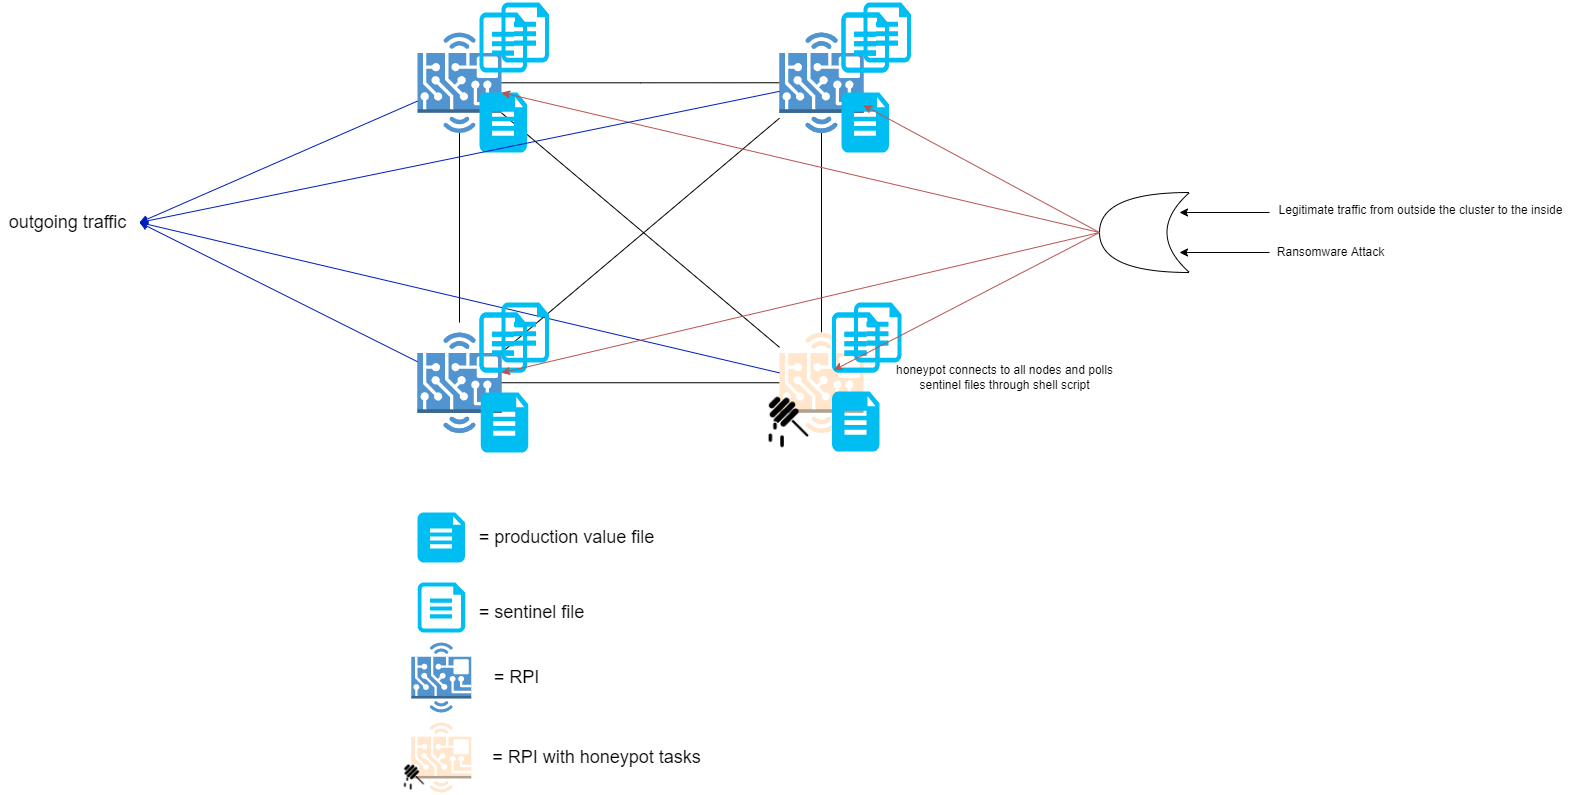
\includegraphics[width = 16cm]{images/ramsonwareHoneypot.png}
  \caption{ Examle scenario of honypot against ramsonware attacks.}
  \label{fig:irradiances}
\end{figure}
\FloatBarrier

\noindent Most IoT solutions include devices that collect data from the environment and send it to more powerful components that gather such information, possibly perform computation and forward data elsewhere.\\
Any Raspberry Pi in the picture represents a server, each connected to more clients (not shown in the picture). Such servers are then connected among each other through a network and a communication protocol.\\
In this example, the architecture of the network is a full mesh, implying that each server is directly connected to any other. You could think of this network as either a local area network (LAN) or wide area network (WAN). They offer two different flavors of the same problem since in LANs you assume that all devices belonging to the network own a different local IP address and you should deal with the NAT system, while in a WAN servers have different public IP addresses and you should deal with DNS in order to communicate with each node in the network. \\ 
Here, the traffic entering the network can be either legitimate or a ransomware attack, benign or malign respectively.\\
As to the communication protocol, IoT systems mainly rely on REST or MQTT. In this context we could think of servers as MQTT subscriber \& publisher (at the same time), since each server is supposed both to receive and send data. The MQTT broker is the entity through which any data packet has to pass to be forwarded from the publisher to the subscriber.\\
Even though the underlying hardware is the same for each of the servers, one of them plays a different role: it behaves as a malware honeypot.\\
All raspberry devices store two distinct types of files: production value files and sentinel files.
Sentinel files are spread in the network with the sole purpose of being a bait for ransomware. Such files are useless for production, thus no any trusted node in the network should change their content. Any change should be assumed as malicious.\\
The task of the honeypot is to monitor the hash digest of sentinel files. If it changed, then there is a very high chance of being under ransomware attack (since sentinel files do not provide production value and therefore are useless for any legitimate operation).\\
A rudimentary script that analyses differences on sentinel files could be the following:\\
%\begin{tabbing}
%\footnotesize\texttt{if ((Get-FileHash "./baitFile.txt").hash -ne (Get-FileHash "./baitFile.txt").hash)\\ {\> stop-service "serviceName" -force} }\\\\
%\texttt{if ((\=Get-FileHash "./baitFile.txt").hash -ne (Get-FileHash "./baitFile.txt").hash)
%\> stop-service "serviceName" -force}
%\end{tabbing}
Heuristics are available since studies show that ransomware tend to encrypt files starting in alphabetical order (or inverse alphabetical order), thus you can name the sentinel files accordingly. As an example, placing files called "\#\#\#aBaitFile.txt" would be among the first ones to be encrypted with an alphabetical attack.\\
The computation of hash digests with respect to checking the whole content is a clear advantage regarding speed.\\
If a difference in the hash digest is present, then a response takes place. The most straightforward response is the shutdown of communication in the whole network and the insertion of the attacker's IP in a blacklist, denying its upcoming traffic.\\
%While some studies raised doubts about the efficiency of such a simple honeypot, it is worth reminding that it comes at zero cost and therefore is a valuable option because the placement of a honeypot is an improvement on no monitoring at all, as every study agrees.\\
%As to the ransomware, we could either think of using a real one exposing the system to a real threat or deploy some simulated, ad-hoc malware. Some material is available online regarding the creation of simple ransomware via PowerShell, as reported in link {[19]} of the Appendix.
An improvement with respect to the scenario depicted above could be the deployment of multiple honeypots at the same time, allowing more servers to monitor sentinel files.\\
The proof of concept can be constructed thanks to a simulated ransomware attack. Some material is available online regarding the creation of simple ransomware via PowerShell, as reported in "How to: Simulating A Ransomware Attack With PowerShell" \cite{Howto}.



\section{Case of study 2: Cluster and Honeypot for a DoS attack}

In the paper named \textit{Use of Honeypots for Mitigating DoS Attacks 
targeted on IoT Networks}\cite{7944057} we found an analysis of the usage of a honeypot to reduce the damage of a DOS attack. One of the several possible attacks on IoT 
systems, Denial of Service (DoS) attack has been a nightmare for 
communication networks over the years and they 
pose a major security threat to IoT systems as well.\\

\subsection{Structure of the IoT cluster for the project}
In order to create the honeypot and check if it works, we would need to create the IoT "cluster" and the DoS client. It is a good idea to start with the most possible structure, and if we manage to create it without any particular difficulty, we could make it more realistic and more complex. So our simple IoT cluster could have very different implementations. We had many ideas, the first of which is reported in the figure below.\\

\begin{figure}[h!]
  \centering
  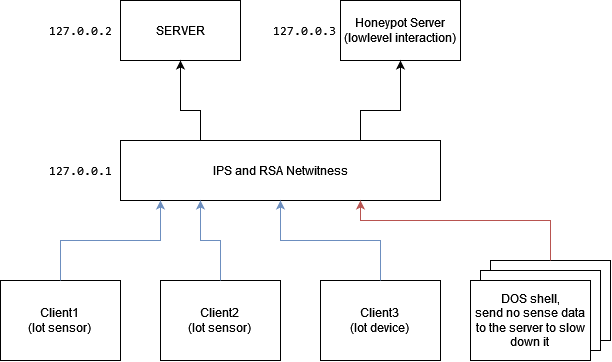
\includegraphics[width = 15cm]{images/IOTIPS.drawio.png}
  \caption{IoT network scheme with IPS.}
  \label{fig:2period}
\end{figure}
\FloatBarrier

An Intrusion Prevention System (IPS) is an active protection system. It attempts to identify potential threats based upon monitoring features of a protected host or network and can use signature, anomaly, or hybrid detection methods. Unlike an Intrusion Detection System, an IPS takes action to block or remediate an identified threat. While an IPS may raise an alert, it also helps to prevent the intrusion from occurring. An IDS is a passive monitoring solution for detecting cybersecurity threats to an organization. If a potential intrusion is detected, the IDS generates an alert that notifies security personnel to investigate the incident and take remedies against the action. \\
In our first proposal the system is less complex, because the IPS itself takes the decision on where to redirect the traffic to. If it is a malicious one, to the honeypot that will collect data about it, if it is a normal one, to the server. The IPS needs time to take decisions, so the traffic could be slowed down by it. If the application doesn't require high availability, this solution is acceptable.
Our second idea is reported in figure below.

\begin{figure}[h!]
  \centering
  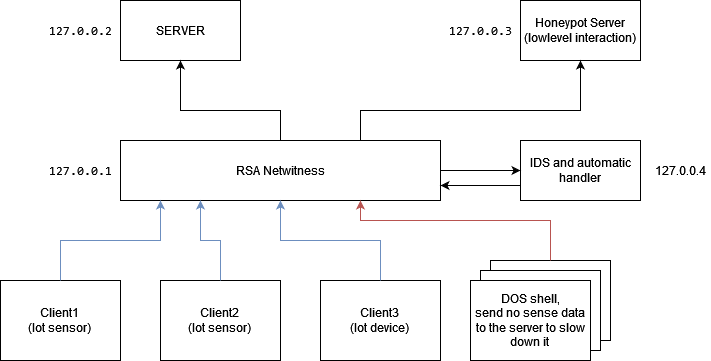
\includegraphics[width = 15cm]{images/IOTIDS.drawio.png}
  \caption{IoT network scheme with IDS.}
  \label{fig:1period}
\end{figure}
\FloatBarrier

This time an ad-hoc server has an IDS, that arises an alarm when something wrong is happening. Then an algorithm inside the server takes a decision on what to do with this possible malicious connection, and sends a command to the RSA server to redirect the traffic. In this way, the system has an high availability because the RSA server is not slow down by the IDS, that acts in a totally autonomous way. However, this idea requires more engineering effort and hardware. If the implementation of these two systems takes less time than expected, we could try to create a more realistic IoT cluster like in the figure below.
\begin{figure}[h!]
  \centering
  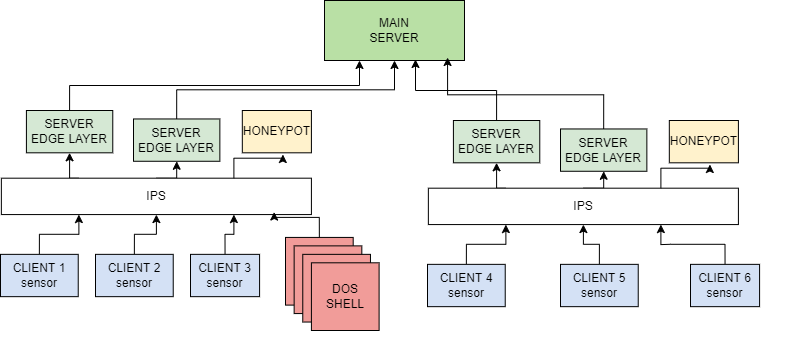
\includegraphics[width = 15cm]{images/IOTlevel2IPS.drawio.png}
  \caption{IOT network scheme level 2 with IPS}
  \label{fig:3period}
\end{figure}
\FloatBarrier
\noindent If we didn't manage to to that, we could see this last idea as a possible future implementation.

\subsection{DOSPOTPY and climatOffice}
In the last years it becomes more and more important to avoid waste of energy at home and at work, due to the increasing cost of energy and to the environmental impact from the chain of the energy supply. So a startup develop a new IoT system named climatOffice(This is only an imaginary company, it doesn't exist in the real life). This solution aims at control the temperature in every office of the company, using N temperature sensors in every room an at least one air conditioner. The desired temperature could be set by an external terminal to the server that control every room. If there are windows in the room, the system also offer the possibility to control the illumination using automatics roll-up shutter. The last feature of this IoT cluster is to possibly control the accesses to some vulnerable rooms, like the server's farm room. So it can lock or unlock some doors. It can do this last thing automatically or by a command from a terminal. A possible structure of this system is reported in the picture below.
\begin{figure}[h!]
  \centering
  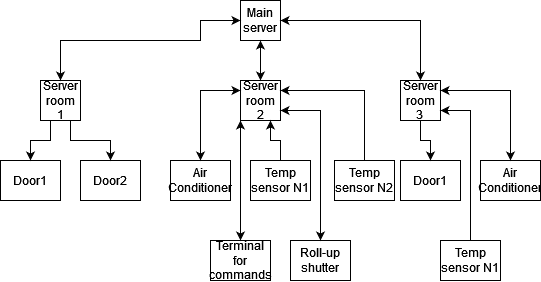
\includegraphics[width = 10cm]{images/climatOffice.drawio.png}
  \caption{An example of the climatOffice IoT cluster}
  \label{fig:TCPDos}
\end{figure}
\FloatBarrier
\noindent
A possible Dos attack could for example avoid the door to close or open, or shut down the air conditioner system. To avoid so we could implement our honeypot and IPS like in the precedent figures. For example, our attacker implement a bot that connect to the system and create thousands of fake temperature sensor that send random and wrong data to the server. Our IPS usually send new traffic connection to the honeypot, that will analyse the data . If this is no sense data, the honeypot will store in a log file the IP addresses of the fake sensor and will told to the IPS to close the connections and to avoid accept new one from that IP.





%DELETE THIS AT THE END
In this chapter you should provide a general overview of the project, explaining what you have implemented staying at a high-level of abstraction, without going too much into the details. Leave details for the implementation chapter. This chapter can be organized in sections, such as goal of the project, issues to be solved, solution overview, etc.\\It is very important to add images, schemes, graphs to explain the original problem and your solution. Pictures are extremely useful to understand complex ideas that might need an entire page to be explained.\\Use multiple sections to explain the starting point of your project, the last section is going to be the high-level view of your solution...so take the reader in a short `journey` to showcase your work.